%%%%%%%%%%%%%%%%%%%%%%%%%%%%%%%%%%%%%%%%%%%%%%%%%
% openshift.tex
% 
% Latex source to be converted to HTML by tex4ht
%
%%%%%%%%%%%%%%%%%%%%%%%%%%%%%%%%%%%%%%%%%%%%%%%%%
\documentclass{article}

%%%%%%%%%%%%%%%%%%%%%%%%%%%%%%%%%%%%%%%%%%%%%%%%%
% PREAMBLE
%%%%%%%%%%%%%%%%%%%%%%%%%%%%%%%%%%%%%%%%%%%%%%%%%
% Import common configurations and custom functions
%%%%%%%%%%%%%%%%%%%%%%%%%%%%%%%%%%%%%%%%%%%%%%%%%
% PREAMBLE
%%%%%%%%%%%%%%%%%%%%%%%%%%%%%%%%%%%%%%%%%%%%%%%%%
\usepackage{hyperref}
\usepackage{listings}
\usepackage{color}
\usepackage[dvipsnames]{xcolor}
\usepackage{float}
\usepackage{graphicx}
\usepackage{tikz,tikz-dependency}
\usepackage{ifthen}
\usetikzlibrary{calc}
\usetikzlibrary{automata,positioning,external,shapes,arrows,chains,matrix,scopes,backgrounds}

% The following is for tikz externalization configuration which allows
% tikZ diagrams to render correctly while being processed by htlatex 
% http://tex.stackexchange.com/questions/158551/using-htlatex-with-tikz-dependency#158921
%%%%%%%%%%%%%%%%%%%%%%%%%%%%%%%%%%%%%%%%%%%%%%%%%
\tikzset{
    tex4ht inc/.style={
        /pgf/images/include external/.code={%
            \includegraphics[]{##1.svg}%
        }

    }
}
\tikzset{
 external/system call/.add={}
      ; inkscape -z -f "\image.pdf" -l "\image.svg"
}
\makeatletter
\@ifpackageloaded{tex4ht}{
    \tikzexternalize[mode=only graphics]
}{
    \tikzexternalize
}
\makeatother

% Removes section numbers
\makeatletter
\renewcommand\thesection{}
%\renewcommand\thesubsection{\@arabic\c@section.\@arabic\c@subsection}
\renewcommand\thesubsection{}
\makeatother

% lstlisting configs for code syntax formatting
\lstdefinestyle{Java} {
  frame=tb,
  language=Java,
  aboveskip=3mm,
  belowskip=3mm,
  showstringspaces=false,
  columns=flexible,
  basicstyle={\large\ttfamily},
  numbers=none,
  numberstyle=\textcolor{gray},
  keywordstyle=\textcolor{red!75},
  commentstyle=\textcolor{dkgreen},
  stringstyle=\textcolor{blue},
  moredelim=[is][\textcolor{black!75}]{|}{|},
  breaklines=false,
  breakatwhitespace=true,
  tabsize=3
}
%%%%%%%%%%%%%%%%%%%%%%%%%%%%%%%%%%%%%%%%%%%%%%%%%
% COLOR DEFINITIONS
%%%%%%%%%%%%%%%%%%%%%%%%%%%%%%%%%%%%%%%%%%%%%%%%%
\tikzstyle{red}     = [fill=red!30!white]
\tikzstyle{orange}  = [fill=orange!30!white]
\tikzstyle{yellow}  = [fill=yellow!30!white]
\tikzstyle{green}   = [fill=green!30!white]
\tikzstyle{blue}    = [fill=blue!30!white]
\tikzstyle{teal}    = [fill=teal!30!white]
\tikzstyle{purple}  = [fill=purple!30!white]
\tikzstyle{magenta} = [fill=magenta!30!white]
\tikzstyle{gray}    = [fill=gray!30!white]
\tikzstyle{black}   = [fill=black!30!white]

%%%%%%%%%%%%%%%%%%%%%%%%%%%%%%%%%%%%%%%%%%%%%%%%%
% DEFINE STACK COLORS
%%%%%%%%%%%%%%%%%%%%%%%%%%%%%%%%%%%%%%%%%%%%%%%%%
\definecolor{DEFINE_USR_COLOR}{HTML}{006699}
\definecolor{DEFINE_KRN_COLOR}{HTML}{003366}
\definecolor{DEFINE_HW_COLOR}{HTML}{000033}
\definecolor{DEFINE_CET_COLOR}{HTML}{339999}

\tikzstyle{DK_COLOR}  = [fill=blue!30!white]
\tikzstyle{ARQ_COLOR} = [fill=gray!30!white]
\tikzstyle{OS_COLOR}  = [fill=black!50!white]
\tikzstyle{USR_COLOR} = [fill=DEFINE_USR_COLOR]
\tikzstyle{KRN_COLOR} = [fill=DEFINE_KRN_COLOR]
\tikzstyle{HW_COLOR}  = [fill=DEFINE_HW_COLOR]
\tikzstyle{CET_COLOR} = [fill=DEFINE_CET_COLOR]
\tikzstyle{HM_COLOR}  = [fill=cyan!30!white]
%%%%%%%%%%%%%%%%%%%%%%%%%%%%%%%%%%%%%%%%%%%%%%%%%
% STACK DIAGRAM DEFINITIONS
%%%%%%%%%%%%%%%%%%%%%%%%%%%%%%%%%%%%%%%%%%%%%%%%%
\tikzstyle{layer}      = [rectangle, thick, rounded corners]
\tikzstyle{core_stack} = [layer, minimum width=11cm,minimum height=1cm, text = white]
\tikzstyle{user_stack} = [layer, minimum width=4cm,minimum height=1cm]
\tikzstyle{app_stack}  = [layer, minimum width=4.5cm,minimum height=3cm]
\tikzstyle{container}  = [layer, purple,minimum width=0.5cm,minimum height=0.5cm]

\tikzstyle{OS_LAYER}  = [app_stack, mw, OS_COLOR, label={[label distance=-0.75cm]270:OpenShift}]
\tikzstyle{ARQ_LAYER} = [app_stack, ARQ_COLOR,label={[label distance=-0.75cm]270:Arquillian}]
\tikzstyle{CET_LAYER} = [user_stack, CET_COLOR]
\tikzstyle{USR_LAYER} = [core_stack, USR_COLOR, minimum height=4.5cm, label={[label distance=-0.75cm]270:\color{white}Userspace}]
\tikzstyle{KRN_LAYER} = [core_stack, KRN_COLOR, below= 0cm of USR]
\tikzstyle{HW_LAYER}  = [core_stack, HW_COLOR, below of=KRN]
\tikzstyle{DK_LAYER}  = [user_stack, DK_COLOR]
\tikzstyle{HM_LAYER}  = [user_stack, HM_COLOR]

%%% NEW DEFS
\tikzstyle{OS_LAYER2} = [app_stack, OS_COLOR,fill=black!50!white, label={[label distance=-0.75cm]270:OpenShift}]


\tikzstyle{c_temp} = [layer,minimum width=0.5cm,minimum height=0.5cm]
\tikzstyle{c_empt} = [c_temp]
\tikzstyle{c_move} = [c_temp, draw, dotted]
\tikzstyle{c_full} = [c_temp, purple, draw=black, thin]
\tikzstyle{mw}     = [minimum width=5.0cm]

%%%%%%%%%%%%%%%%%%%%%%%%%%%%%%%%%%%%%%%%%%%%%%%%
% Tikz Functions
%%%%%%%%%%%%%%%%%%%%%%%%%%%%%%%%%%%%%%%%%%%%%%%%
\newcommand{\moby}[4] {
  \xdef\cmax{7}
  \def\id{#1}                   % #1 = id 
  \pgfmathsetmacro\nc{int(#2)}  % #2 = number of containers
  \pgfmathsetmacro\nfc{int(#3)} % #3 = number of full containers 
                                % #4 = location
  % Initialize container nodes
  \foreach \x in {0,...,7}{
    \node[] (C\x_\id) {};
  }
  % Instantiate moby and container nodes
  \node[DK_LAYER, DK_COLOR, #4] (DK_\id) {Moby};
  \node[above left= 0.1cm and 0cm of DK_\id.north west] (sp) {};

  \xdef\sp{sp};     % starting position
  \xdef\ct{c_full}; % container type
  \foreach \x in {0,...,\cmax} {
    {\ifthenelse{\x < \nc}
      { {\ifthenelse{\x < \nfc }
          {\xdef\ct{c_full};}
          {\xdef\ct{c_move};}
        }
      }
      { \xdef\ct{c_empt};}
    }
    \node[\ct, right=of \sp] (C\x_\id) {};
    \xdef\sp{C\x_\id};
  };

  {\ifthenelse{\nc < 4}{}{
  %Container label with spanning arrows 
  \node[above= 0.5cm of DK_\id.north ] (C_LABEL_\id) {Containers};
  \path[->, to path={-| (\tikztotarget)}]
  (C_LABEL_\id.west) edge (C0_\id.north)
  (C_LABEL_\id.east) edge (C7_\id.north);
  }};
}
\newcommand{\host}[4]{
  \def\id{#1}  % #1 = id
  \def\nc{#2}  % #2 = number of containers
  \def\nfc{#3} % #3 = number of full containers
               % #4 = location
  % Initialize nodes
  \foreach \x in {0,...,7}
    \node[] (C\x_\id) {};
    \node[] (DK_\id) {};
    \node[] (OS_\id) {};

  \node[OS_LAYER,fit=(DK_\id)] at (#4) (OS_\id) {};
  \moby{#1}{#2}{#3}{above = 0cm of OS_\id.center, anchor=center};
  \node[HM_LAYER, mw, below= 0cm of OS_\id.south, anchor=north] (HM_\id) {Host Machine \id};
}

\newcommand{\OpenShift}[4]{
  \def\id{#1}  % #1 = id
  \def\nc{#2}  % #2 = number of containers
  \def\nfc{#3} % #3 = number of full containers
               % #4 = location
  % Initialize nodes
  \foreach \x in {0,...,7}
    \node[] (C\x_\id) {};
    \node[] (DK_\id) {};
    \node[] (OS_\id) {};

  \node[OS_LAYER,fit=(DK_\id), #4] (OS_\id) {};
  \moby{#1}{#2}{#3}{above = 0cm of OS_\id.center, anchor=center};
}

\newcommand{\Arquillian}[2]{
  \def\id{#1}  % #1 = id
               % #2 = location

  \node[] (CET_\id) {};
  \node[ARQ_LAYER, fit=(CET_\id), #2] (ARQ_\id) {};
  \node[CET_LAYER, above = 0cm of ARQ_\id.center, anchor=center] (CET_\id) {CE-Testsuite};
}

\newcommand{\pods}[5]{
  \xdef\id{#1}
  \pgfmathtruncatemacro{\numPods}{#2-1}
  \xdef\numCons{#3-1};
  \pgfmathtruncatemacro{\cpp}{2 - 1} %containers per pod
  \xdef\cfit{} % containers for pod to fit
  \xdef\pfit{} % pods for namespace to fit

  \node[#4] (BASE) {};
  \xdef\lcp{BASE}; % last container position
  \xdef\sbc{}; % space between container
  \pgfmathsetmacro\r{#3}
 % Initialize pods
  \foreach \x in {0,...,\numPods}{
    \pgfmathsetmacro\pods{int(#2 - \x))}
    {\ifthenelse{\r > \pods }
    { % if 
      \xdef\numCons{1}
      \pgfmathsetmacro\r{int(\r - 2)}
      \xdef\r{\r}
    }
    { % else
      \xdef\numCons{0};
      \pgfmathsetmacro\r{int(\r - 1)}
      \xdef\r{\r}
    }
    };
    %\node[] at (-5,\x) {\r \pods \numCons};

    \foreach \y in {0,...,\numCons}{
      \node[c_full, right= \sbc of \lcp] (P\x_C\y_#1) {};
      \xdef\lcp{P\x_C\y_#1}
      \xdef\cfit{\cfit(P\x_C\y_#1)} % add container to be fitted
      \xdef\sbc{}; %space between containers
    }

    % randomly generate color for pod
    \pgfmathparse{rnd}
    \pgfmathtruncatemacro{\cc}{(\id)*0.4}
    \xdefinecolor{rColor}{rgb}{\cc, 0.7, \pgfmathresult}

    \node[pod, fill=rColor, fit=\cfit] (P\x_\id) {};
    %\pgfmathparse{rnd * \x}

    \xdef\cfit{};
    \xdef\sbc{0cm and 0.5cm}; %space between containers
    \xdef\pfit{\pfit(P\x_\id)} % add container to be fitted
    }
    #5
}

\newcommand{\namespace}[4]{
  \pods{#1}{#2}{#3}{#4}{\node[fit=\pfit] (NS_#1) {};};
  \node[NS, fit=\pfit] (NS_#1) {};
  \node[above=0cm of NS_#1.north] (NS_#1_LABEL) {Namespace #1};
  %\node[NS, fill=gray!10, fit=\pfit] (NS_#1) {};
  \pods{#1}{#2}{#3}{#4}{};
  %\pods{#1}{#2}{#3}{#4}{};
}


%%%%%%%%%%%%%%%%%%%%%%%%%%%%%%%%%%%%%%%%%%%%%%%%%
% DOCUMENT
%%%%%%%%%%%%%%%%%%%%%%%%%%%%%%%%%%%%%%%%%%%%%%%%%
\begin{document}

\centerline{\sc \large OpenShift}
\centerline{\sc Architecture for the Layperson }
\centerline{\url{https://github.com/openshift/origin}}

\vspace{1pc}

\section{Overview}

\hspace{3pc} Platform as a Service is a clich\'e that is commonly used to describe software which facilitates the 
creation of more software. If OpenShift is similair to a an inn which cleans itself. Sentencing its subjects to death.
Basically, it automates the role of a system administrator. 


\begin{figure}
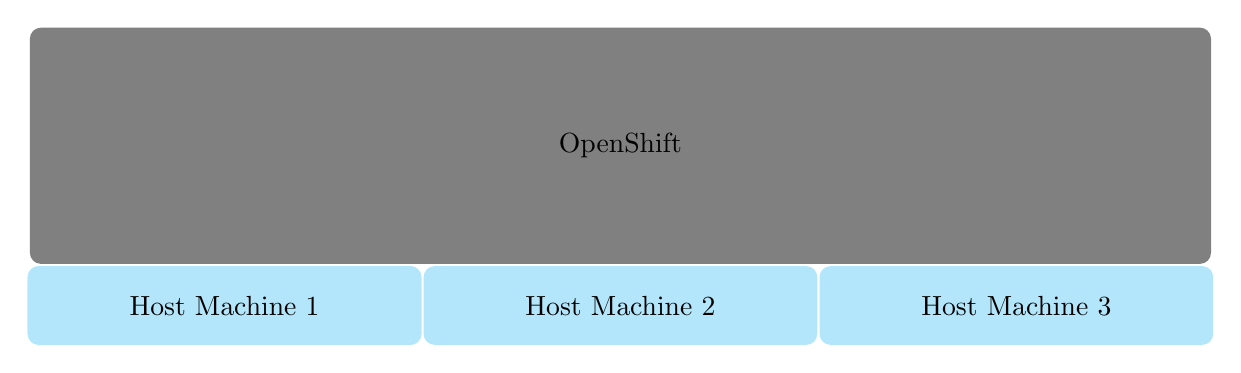
\begin{tikzpicture}[node distance = 1cm and 0cm]
  % OpenShift layer
  \tikzstyle{OS_LAYER} = [app_stack, OS_COLOR, minimum width = 15cm]

  \node[HM_LAYER, mw] (HM_1) {Host Machine 1};
  \node[HM_LAYER, mw, right=of HM_1] (HM_2) {Host Machine 2};
  \node[HM_LAYER, mw, right=of HM_2] (HM_3) {Host Machine 3};
  \node[OS_LAYER, above=0cm of HM_2] (OS_1) {OpenShift};
  \node[HM_LAYER, mw] (MB_1) {Host Machine 1};
  %\node[HM_LAYER, mw, below= 0cm of DK_1.south, anchor=north] (HM_1) {Host Machine 1};
  %\node[HM_LAYER, mw, below= 0cm of DK_1.south, anchor=north] (HM_1) {Host Machine 1}; 
\end{tikzpicture}
\end{figure}

\section{Pods and Services}
The core components which an application is build upon are pods and services. The whole purpose of container platforms
is to relief programmers of mundane task of environmental upkeep. Pods are an abstraction of a programmer's computing environment
hence, the platform part of platform of a service. A pod is just a grouping of isolated processes that emulate a virtual 
operating system. A pod is just a grouping of isolated processes that emulate a virtual operating system  
%\iffalse
%Distributed openshift and pod diagram
%%%%%%%%%%%%%%%%%%%%%%%%%%%%%%%%%%%%%%%%%%%%%%%%%
% Anatomy of a Pod
%%%%%%%%%%%%%%%%%%%%%%%%%%%%%%%%%%%%%%%%%%%%%%%%%
\begin{figure}
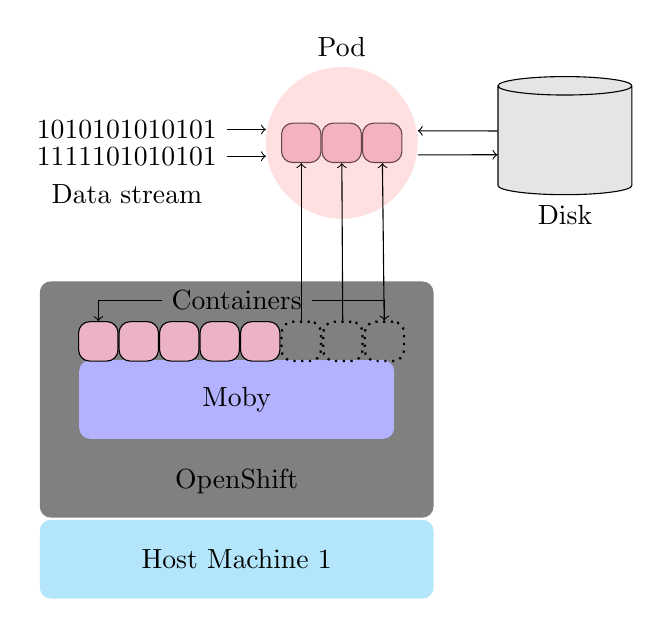
\begin{tikzpicture}[node distance = 1cm and 0cm]
  \tikzstyle{pod}= [thick, opacity=0.4, rounded corners, circle]

  \host{1}{8}{5}{0,0};

  %%%%%%%%%%%%%%%%%%%%%%%%%%%%%%%%%%%%%%%%%%%%%%%%%
  % POD DIVISION
  %%%%%%%%%%%%%%%%%%%%%%%%%%%%%%%%%%%%%%%%%%%%%%%%%
  % pods
  \node[c_full, above= 2cm of C5_1]  (P1)        {};
  \node[c_full, right= of P1]        (P2)        {};
  \node[c_full, right= of P2]        (P3)        {};
  \node[pod,fill=red!30!white, fit=(P1)(P2)(P3)] (pod) {};
  \node[above= 0cm of pod] (pod_label) {Pod};

  \path[->] (C5_1) edge (P1);
  \path[->] (C6_1) edge (P2);
  \path[->] (C7_1) edge (P3);

  \node[left= 0cm and 0.5cm of pod.170] (data_flow) {1010101010101};
  \node[left= 0cm and 0.5cm of pod.190] (data_flow2) {1111101010101};
  \path[->] (data_flow.east) edge (pod.170);
  \path[->] (data_flow2.east) edge (pod.190);
  \node[below= 0cm of data_flow2] (net_label) {Data stream};

  \tikzstyle{d_seg_color} = [fill=black!10]
  \tikzstyle{d_seg} = [cylinder, d_seg_color,draw, shape border rotate=90, thin, minimum width = 1.7cm, minimum height = 1.5cm]

  \node[d_seg, right= 0.0cm and 1cm of pod.east] (D0) {};
  \node[below= 0cm of D0 ] (D0_label) {Disk};

  \path[->] (D0.170) edge (pod.9);
  \path[<-] (D0.190) edge (pod.351);

\end{tikzpicture}
\caption{Anatomy of a Pod}
\end{figure}


\section{Container Registry}
OpenShift is able to store the blueprints for applications in what is know as a registry

\section{Build}

\section{Image Stream}
"Comprises of any number of container images identified by tages / Virtual view of related images"
A collection of image references, a way to mass import container images into OpenShift
Keeps track of images within registry

importing a tag or image into an image stream?

\section{TODO}
\begin{enumerate}
  \item Pods and Services
  \item Builds and Image Streams
  \item Container Registry
  \item Web console
  \item Builds and Image Streams
  \item Deployments
  \item Templates
\end{enumerate}


\end{document}

